\section{Sojowe kotlety mielone}
\bigskip
\small
\begin{minipage}{0.45\textwidth}
    \noindent \textbf{Czas:} 30 minut \\
    \textbf{Poziom trudności:} umiarkowany
\end{minipage}
\begin{minipage}{0.45\textwidth}
    \noindent \textbf{Ilość sprzątania:} średnia\\
    \textbf{Wymagany mysi sprzęt:} -
\end{minipage}
\normalsize
\vspace{0.5cm}

\begin{multicols}{2}

\subsection*{Składniki}
\begin{itemize}
    \item 150 g granulatu sojowego
    \item 30 g ugotowanej kaszy jaglanej
    \item 500 ml wrzątku
    \item 1-2 łyżki bulionu warzywnego/drobiowego/wołowego ze słoiczka
    \item 1/2 cebuli
    \item 1 jajko
    \item 3 łyżki przyprawy do mięsa mielonego
    \item 3 łyżki bułki tartej + kilka łyżek do panierowania
    \item 2 łyżki musztardy
    \item 1 łyżeczka koncentratu pomidorowego
    \item 2 łyżki oleju + do smażenia
    \item sól i pieprz do smaku
\end{itemize}

\columnbreak

\begin{figure}[H]
    \centering
    \fbox{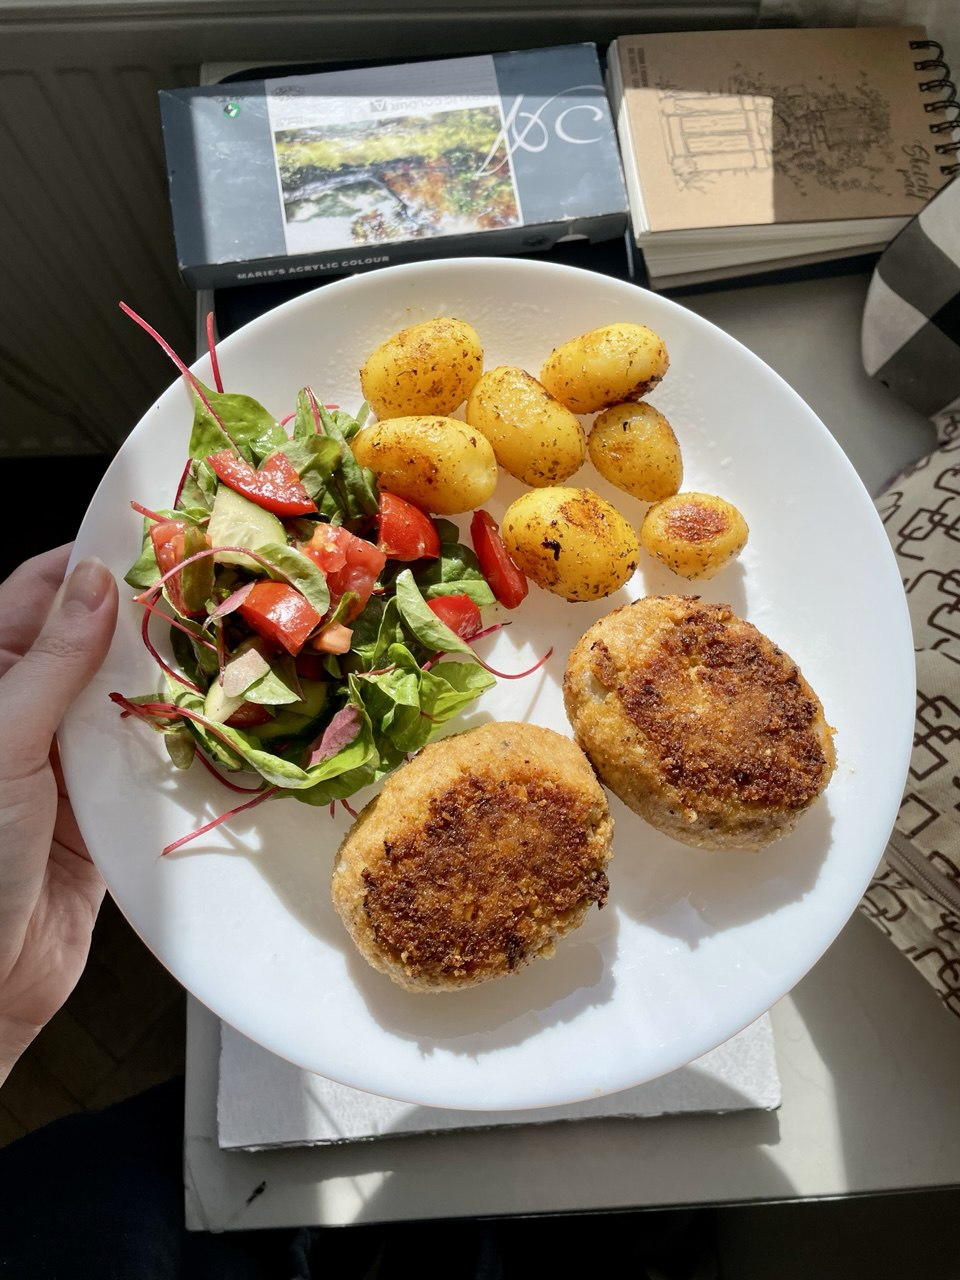
\includegraphics[width=0.4\textwidth]{images/mielone.jpg}}
\end{figure}
\end{multicols}

\vspace{0.5cm}

\subsection*{Instruktaż}
\begin{enumerate}
    \item Kaszę jaglaną ugotować zgodnie z instrukcją na opakowaniu, ale bez soli. W międzyczasie wsypać do średniej miski granulat sojowy, zalać wrzątkiem i wymieszać dokładnie razem z bulionem. Odstawić pod przykryciem na 10 minut.
    \item Cebulę pokroić w bardzo drobną kostkę i wrzucić do dużej miski wraz z ugotowaną i lekko ostudzoną kaszą jaglaną, olejem, koncentratem pomidorowym przyprawą do mielonego i musztardą.
    \item Przestudzony granulat odcedzić na sitku lub mocno w dłoniach i dorzucić do dużej miski z cebulą. Wszystko dokładnie wymieszać i sprawdzić smak pod kątem soli oraz pieprzu.
    \item Dodać jajko oraz bułkę tartą i dokładnie wymieszać. Jeżeli konsystencja jest zbyt kleista/mokra do lepienia kotletów, dodać więcej bułki tartej, a jeżeli zbyt sucha, to odrobinę więcej bulionu pozostałego z odciskania granulatu.
    \item Rozgrzać mocno olej na średniej wielkości patelni. Na głęboki talerz lub do miski wsypać bułkę tartą do panierowania.
    \item Do uformowania jednego kotleta dobrze sprawdza się około garść masy. Przed wrzuceniem na patelnię każdego kotleta obtoczyć dokładnie w bułce tartej i smażyć po kilka minut na stronę do uzyskania złoto-brązowego koloru z każdej strony.
\end{enumerate}

\vspace{0.5cm}

\small
\subsection*{Propozycja podania}
Z ubijanymi lub pieczonymi ziemniaczkami, domową mizerią, buraczkami zasmażanymi lub sałatką.

\vspace{0.3cm}

\subsection*{Dodatkowe uwagi}
\begin{itemize}
    \item w wielu przyprawach do mięsa mielonego głównym składnikiem jest sól --- trzeba więc uważać z dodawaniem soli do innych składowych kotletów i przed dodaniem surowego jajka próbować, czy masa nie jest zbyt słona
    \item kotlety można bardzo łatwo przerobić na wegańskie; dobrym zamiennikiem jajka jest łyżeczka nasionek chia zalanych dwiema łyżeczkami wody kilka godzin wcześniej
    \item w celu uzyskania bardziej ,,mięsnego'' smaku najlepiej wybrać bulion na bazie mięsa; można też opcjonalnie dodać składniki typu sos sojowy czy pasta miso, aczkolwiek są to składniki typowo słone, a z nimi trzeba ostrożnie
\end{itemize}

\newpage
